% Supplementary material for the LiSA CVPR 2027 submission (compiled separately from main.tex).
\documentclass[10pt,twocolumn,letterpaper]{article}
\usepackage[review]{cvpr}
%% Preamble for the LiSA CVPR 2027 submission.
%% Based on preamble.tex of the official cvpr-org/author-kit (main branch); only additions below.

%% Official support for 2-column teaser figure
\usepackage{cuted} %< for strip environment
\usepackage{currfile} %< for \currfilebase macro
\usepackage{caption} %< for "\captionof" commands (teaser)

%% Tables and figures
\usepackage{multirow}
\usepackage{tikz}
\usetikzlibrary{positioning,fit,calc,arrows.meta,backgrounds}

%% Text layout (enabled to stay within the page limit without altering the official margins)
\usepackage{microtype}

%% Inline annotations (from the kit). Placeholders for experiments that still have to be run are
%% rendered in red so that they cannot be overlooked; see paper/README.md, "Experiments to run".
\newcommand{\red}[1]{{\color{red}#1}}
\newcommand{\todo}[1]{{\color{red}#1}}
\newcommand{\TODO}[1]{\textbf{\color{red}[TODO: #1]}}
\newcommand{\TBD}{{\color{red}\textbf{TBD}}}
\newcommand{\torun}[1]{{\color{red}\textbf{[TO RUN]} #1}}
%% For the camera-ready / final submission, all \torun and \TBD entries must be resolved.

%% Shorthands
\usepackage{xspace}
\newcommand{\ours}{LiSA\xspace}
\newcommand{\gsthree}{GS$^3$\xspace}
\newcommand{\vect}[1]{\mathbf{#1}}
\DeclareMathOperator{\logit}{logit}
\DeclareMathOperator{\softplus}{softplus}

\definecolor{cvprblue}{rgb}{0.21,0.49,0.74}
\usepackage{xr-hyper}
\externaldocument{../build/main} % main-paper labels (compile main.tex first)
\usepackage[pagebackref,breaklinks,colorlinks,allcolors=cvprblue]{hyperref}
\def\paperID{*****}
\def\confName{CVPR}
\def\confYear{2027}
\title{LiSA: Light-Space Atlases for Relightable Gaussian Splatting}

\begin{document}
\maketitlesupplementary
\renewcommand{\thesection}{S\arabic{section}}
\renewcommand{\thetable}{S\arabic{table}}
\renewcommand{\thefigure}{S\arabic{figure}}
\renewcommand{\theequation}{S\arabic{equation}}

This supplement gives implementation details (\cref{sec:s_impl}), the evaluation protocol and per-scene results (\cref{sec:s_eval}), additional analyses (\cref{sec:s_analysis}), registration and foreground diagnostics (\cref{sec:s_registration}), qualitative results (\cref{sec:s_qual}), and the protocols of the experiments that are still to be run (\cref{sec:s_torun}).
Section, table and equation numbers without the prefix ``S'' refer to the main paper.

\section{Implementation details}
\label{sec:s_impl}

\paragraph{Light camera.}
For every light we build a look-at camera from the light position $\vect p$ to the scene center $\vect c$.
Its half field of view is the 99.9th percentile, over all Gaussians in front of the light, of the angular extent of their $3\sigma$ footprints, enlarged by 5\% and capped at $75^\circ$; distant floaters may therefore fall outside the atlas.
Depths are measured along the optical axis, relative to $\|\vect c-\vect p\|$, and divided by the scene radius $R$, which is estimated from the training cameras.
The texel size $\tau_0$ is the width of one atlas texel at the depth of the scene center, in units of $R$, and $\tau_k=2^k\tau_0$.
The light pass uses gsplat's classic rasterization mode (per-tile sorting by center depth, a 0.3-pixel screen-space dilation, opacities clamped at 0.99 and early ray termination), and each Gaussian contributes the depth of its center.
Over 40 training lights per scene, the atlas half-angle is 8--30$^\circ$ (scene medians 8--23$^\circ$) and never reaches the cap; light distances are 2.0--6.2 scene radii, nearly constant within the synthetic scenes (2.8--3.5 on \gsthree, 2.3 on SSS-GS) and varying by up to $1.8\times$ within a real capture.

\paragraph{Pyramid and gather.}
Each level applies a separable $[1,4,6,4,1]/16$ filter with zero padding and $2\times2$ average pooling.
Receivers sample every level bilinearly with zero padding, so points outside the light frustum see zero coverage and are treated as lit.
In the descriptor, $t_k$ is divided by four and clamped to $[-2,2]$, and $\delta_k$ is multiplied by four and clamped to $[-4,4]$; $M_{0,k}$ is clamped to $[0,1]$ and the mean depth uses $\max(M_{0,k},10^{-4})$ in the denominator.
The logit in \cref{eq:visibility} is evaluated on $V_0$ clamped to $[10^{-4},1-10^{-4}]$.

\paragraph{Networks.}
All networks are MLPs with SiLU activations.
The flux encoder $\mathrm{MLP}_\phi$ has two hidden layers of width 32 and its output bias is initialized to $\softplus^{-1}(1)$.
The visibility residual $g$ has two hidden layers of width 64 with a zero-initialized output layer.
The transfer network $h$ has two hidden layers of width 128 and outputs $K\cdot3\cdot C=168$ values; its output bias is $-7$, so that $L_{\mathrm{tr}}\approx0$ at the start.
The material network has four hidden layers of width 128 and outputs nine RGB responses (one base and eight basis responses); its inputs are the code $\vect f$, the normal, four-band Fourier encodings of $\vect l,\vect v,\vect h$ and the reflected view direction, five cosines ($\vect n\cdot\vect l$, $\vect n\cdot\vect v$, $\vect n\cdot\vect h$, $\vect v\cdot\vect h$, $\vect l\cdot\vect v$) and five highlight hints with $\kappa\in\{8,32,128,512,2048\}$.
The eight light-independent coefficients come from a two-layer MLP of width 64 on $\vect f$ and an eight-band positional encoding, with a zero-initialized output; the lobe weights of $s(\vect x)$ come from a network of the same shape with output bias $-6$.
The normal channels of $\vect f$ are detached wherever $\vect f$ enters a network as a latent code, so the learned normals receive gradients only through the directional terms in which they appear (cosines, the reflected view direction and the $\vect n\cdot\vect l$ input of the flux encoder).

\paragraph{Optimization.}
Densification uses the screen-space gradient rule of 3DGS (threshold $2\cdot10^{-4}$) from iteration 500 to 25k, with opacity resets every 3k iterations and a cap of 400k Gaussians.
During the first 2k iterations, pixels outside the ground-truth mask supervise only coverage.
Like all baselines, \ours processes one training image per iteration.
LDR images (real captures, SSS-GS) are linearized with $\gamma=2.2$; clipped highlights stay clipped, and the HDR \gsthree images are used as provided.
The light pass is first used after the warm-up, i.e., at iteration 8001.
In stage III, the networks start from their stage-II weights with fresh optimizer state; geometry, cameras and the light normalization are frozen.

\paragraph{Real captures.}
For each training camera we optimize a rotation about its calibrated optical center, starting at iteration 2k with a learning rate decayed from $10^{-3}$ to $10^{-5}$.
With fixed centers and free rotations, a global translation of the scene can be absorbed by re-aiming all cameras.
After every camera update we project the rotation corrections off this three-dimensional gauge in closed form and translate the scene by the corresponding offset, which leaves the image position of the object center unchanged in every training view and keeps the reconstruction in the calibrated frame.
Test cameras and lights always use the official calibration.

\section{Evaluation protocol and per-scene results}
\label{sec:s_eval}
Images are evaluated at 512\,px on the longest side (256\,px for SSS-GS).
The \gsthree scenes are linear HDR renderings displayed with $\gamma=2.2$ on a white background; the other benchmarks are displayed as provided on black.
SSIM uses an $11\times11$ Gaussian window ($\sigma=1.5$) with zero padding, and LPIPS uses the VGG network with inputs in $[-1,1]$.
Each method's renderings are compared with one common set of 8-bit targets, namely the test images as encoded by our evaluation pipeline.
The targets produced by the baselines' own pipelines differ from these by at most one intensity level, except on three real captures (CatSmall, CupFabric, Pikachu), where 6--10\% of the channel values of \gsthree, SSD-GS and RNG differ by up to 42 levels.
Re-scoring against the common targets changed per-scene PSNR by at most 0.04\,dB and scene-averaged PSNR by at most 0.005\,dB, and it changed no ranking.
\Cref{tab:perscene} lists all per-scene results.
Across scenes, the advantage of \ours is significant against every baseline under a Wilcoxon signed-rank test ($p=0.004$, 0.007, 0.016 and $<10^{-4}$ against SSD-GS, \gsthree, OLAT-GS and RNG); on the 11 synthetic scenes it is significant against SSD-GS ($p=0.014$) and \gsthree ($p=0.024$) but not against OLAT-GS ($p=0.12$).

\paragraph{Baseline runs.}
All baselines use their released code and default schedules on the official training images, composite their training targets with the provided foreground masks, and render the test views at the official calibration.
Four synthetic SSD-GS models (AnisoMetal, Translucent, Bunny, Dragon) come from earlier runs with the same protocol, without pose refinement, and were re-scored.
Several RNG runs and the OLAT-GS runs on Drums and Lego reach low scores; we have not verified that these reproduce the published behavior of the methods, which experiment E6 addresses.

\paragraph{Use of the benchmarks during development.}
The method was developed on these benchmarks.
Earlier versions (\cref{tab:supp_history}) were evaluated on the official test views, first of Cat, Pixiu, AnisoMetal, Translucent, Bunny and Dragon and later of all 18 scenes, and these results identified the failures on Lego and Drums.
Design choices for the final version were then made on views held out from the training sets: the material network on held-out light groups, and the staged schedule on every tenth training view of Lego, Drums, FurBall, Cat and Soap.
The final configuration was run once on all 18 scenes, with no per-scene settings and no checkpoint selection on test views.
The results should therefore be read as benchmark results of a method developed on these benchmarks rather than as a blind test.

\begin{table*}[t]
\caption{\textbf{Per-scene results} (PSNR$\uparrow$ / SSIM$\uparrow$ / LPIPS$\downarrow$), common targets, original test calibration, seed 0. Best PSNR per scene in \textbf{bold}.}
\label{tab:perscene}
\centering\scriptsize
\setlength{\tabcolsep}{3pt}
\begin{tabular}{@{}llccccc@{}}
\toprule
Benchmark & Scene & RNG & OLAT-GS & GS$^3$ & SSD-GS & \textbf{LiSA (ours)} \\
\midrule
\multirow{7}{*}{NRHints (real)} & Cat & 20.99 / 0.773 / 0.287 & 22.43 / 0.768 / 0.206 & 19.12 / 0.717 / 0.232 & 18.09 / 0.705 / 0.247 & \textbf{25.33} / 0.821 / 0.171 \\
 & CatSmall & 18.74 / 0.792 / 0.212 & 31.58 / 0.949 / 0.081 & 33.28 / 0.967 / 0.076 & \textbf{33.83} / 0.967 / 0.079 & 33.02 / 0.961 / 0.082 \\
 & CupFabric & 21.41 / 0.847 / 0.201 & \textbf{36.40} / 0.979 / 0.049 & 35.16 / 0.976 / 0.053 & 35.98 / 0.979 / 0.054 & 35.31 / 0.976 / 0.059 \\
 & Fish & 24.11 / 0.842 / 0.187 & 23.85 / 0.834 / 0.153 & 22.41 / 0.809 / 0.171 & 23.27 / 0.822 / 0.151 & \textbf{28.97} / 0.896 / 0.111 \\
 & FurScene & 24.12 / 0.861 / 0.162 & 24.77 / 0.868 / 0.113 & \textbf{26.09} / 0.891 / 0.103 & 25.15 / 0.877 / 0.112 & 24.47 / 0.864 / 0.119 \\
 & Pikachu & 17.27 / 0.833 / 0.201 & 31.06 / 0.962 / 0.055 & 31.16 / 0.967 / 0.057 & 30.69 / 0.965 / 0.058 & \textbf{31.65} / 0.967 / 0.056 \\
 & Pixiu & 19.95 / 0.848 / 0.172 & 20.70 / 0.841 / 0.143 & 23.72 / 0.864 / 0.117 & 23.39 / 0.862 / 0.119 & \textbf{26.20} / 0.881 / 0.107 \\
\midrule
\multirow{6}{*}{GS$^3$ (synthetic)} & AnisoMetal & 24.32 / 0.923 / 0.072 & 27.51 / 0.961 / 0.039 & 27.51 / 0.950 / 0.058 & \textbf{28.00} / 0.957 / 0.047 & 27.15 / 0.956 / 0.040 \\
 & Drums & 15.44 / 0.832 / 0.238 & 20.64 / 0.922 / 0.096 & 31.52 / 0.976 / 0.029 & \textbf{31.54} / 0.976 / 0.029 & 30.45 / 0.976 / 0.030 \\
 & FurBall & 17.61 / 0.890 / 0.169 & 35.56 / 0.968 / 0.062 & 35.83 / 0.968 / 0.079 & 35.00 / 0.965 / 0.086 & \textbf{36.11} / 0.971 / 0.054 \\
 & Hotdog & 29.40 / 0.953 / 0.060 & 29.67 / 0.966 / 0.046 & 33.32 / 0.974 / 0.036 & 32.94 / 0.973 / 0.037 & \textbf{35.22} / 0.980 / 0.029 \\
 & Lego & 16.78 / 0.809 / 0.200 & 20.27 / 0.852 / 0.192 & \textbf{30.91} / 0.956 / 0.050 & 29.72 / 0.944 / 0.061 & 30.80 / 0.959 / 0.044 \\
 & Translucent & 29.29 / 0.961 / 0.052 & 29.03 / 0.971 / 0.041 & 32.76 / 0.975 / 0.042 & 31.99 / 0.975 / 0.038 & \textbf{34.67} / 0.981 / 0.031 \\
\midrule
\multirow{5}{*}{SSS-GS (synthetic)} & Bunny & 37.85 / 0.988 / 0.020 & \textbf{40.43} / 0.991 / 0.016 & 34.42 / 0.980 / 0.032 & 38.49 / 0.989 / 0.019 & 39.86 / 0.990 / 0.016 \\
 & Candle & 41.88 / 0.994 / 0.015 & 45.08 / 0.997 / 0.008 & 38.74 / 0.988 / 0.022 & 38.74 / 0.989 / 0.020 & \textbf{45.20} / 0.996 / 0.008 \\
 & Dragon & 35.23 / 0.973 / 0.042 & \textbf{37.79} / 0.982 / 0.026 & 36.10 / 0.977 / 0.032 & 37.38 / 0.982 / 0.027 & 37.38 / 0.981 / 0.026 \\
 & Soap & 40.28 / 0.991 / 0.013 & \textbf{41.42} / 0.992 / 0.011 & 38.35 / 0.984 / 0.027 & 38.36 / 0.988 / 0.022 & 40.91 / 0.992 / 0.012 \\
 & Statue & 30.23 / 0.968 / 0.048 & 38.99 / 0.989 / 0.022 & 36.43 / 0.985 / 0.025 & 35.99 / 0.983 / 0.027 & \textbf{39.82} / 0.989 / 0.020 \\
\bottomrule
\end{tabular}
\end{table*}


\section{Additional analyses}
\label{sec:s_analysis}

\paragraph{Transfer share.}
\Cref{tab:supp_shares} reports, for every scene, the share of linear radiance that the final model routes through the transfer term.
It is lowest on the opaque synthetic objects (5.6\% on Drums to 9.3\% on Lego), higher on fur and the Translucent scene (about 17\%), and highest on the subsurface-scattering scenes (20.5--58.0\%).
On real captures it varies between 7.2\% (FurScene) and 42.1\% (Pixiu, a translucent resin figure); there the transfer term also absorbs effects that the local model cannot explain.
These shares describe how the learned model allocates radiance, not a physical decomposition.

\begin{table}[t]
\caption{\textbf{Transfer share and light novelty per scene.} Share of linear radiance routed through $L_{\mathrm{tr}}$ by the final model (mean and range over 8 evenly spaced test views), mean learned visibility over covered pixels, and the angle between each official test light and the nearest training light (median / maximum).}
\label{tab:supp_shares}
\centering\scriptsize
\setlength{\tabcolsep}{3pt}
\begin{tabular}{@{}llcccc@{}}
\toprule
Benchmark & Scene & Transfer share & Range & Mean $V$ & Test-light novelty \\
\midrule
\multirow{7}{*}{NRHints (real)} & Cat & 34.2\% & 28--44\% & 0.66 & 2.3$^\circ$ / 10.5$^\circ$ \\
 & CatSmall & 26.8\% & 21--40\% & 0.55 & 1.2$^\circ$ / 3.5$^\circ$ \\
 & CupFabric & 19.2\% & 12--25\% & 0.76 & 1.3$^\circ$ / 3.6$^\circ$ \\
 & Fish & 28.2\% & 1--45\% & 0.88 & 2.2$^\circ$ / 8.8$^\circ$ \\
 & FurScene & 7.2\% & 5--11\% & 0.59 & 2.1$^\circ$ / 6.6$^\circ$ \\
 & Pikachu & 12.3\% & 9--20\% & 0.55 & 0.9$^\circ$ / 3.7$^\circ$ \\
 & Pixiu & 42.1\% & 37--45\% & 0.83 & 2.1$^\circ$ / 5.1$^\circ$ \\
\midrule
\multirow{6}{*}{GS$^3$ (synthetic)} & AnisoMetal & 7.4\% & 6--11\% & 0.89 & 1.1$^\circ$ / 3.9$^\circ$ \\
 & Drums & 5.6\% & 4--7\% & 0.77 & 1.1$^\circ$ / 3.9$^\circ$ \\
 & FurBall & 16.9\% & 16--19\% & 0.84 & 1.1$^\circ$ / 3.9$^\circ$ \\
 & Hotdog & 6.7\% & 6--8\% & 0.92 & 1.1$^\circ$ / 3.9$^\circ$ \\
 & Lego & 9.3\% & 7--14\% & 0.75 & 1.1$^\circ$ / 3.9$^\circ$ \\
 & Translucent & 16.7\% & 14--21\% & 0.89 & 1.1$^\circ$ / 3.9$^\circ$ \\
\midrule
\multirow{5}{*}{SSS-GS (synthetic)} & Bunny & 28.1\% & 13--81\% & 0.67 & 0.0$^\circ$ / 11.3$^\circ$ \\
 & Candle & 47.6\% & 28--88\% & 0.49 & 0.0$^\circ$ / 11.2$^\circ$ \\
 & Dragon & 48.2\% & 34--79\% & 0.46 & 0.0$^\circ$ / 11.2$^\circ$ \\
 & Soap & 58.0\% & 32--98\% & 0.63 & 0.0$^\circ$ / 11.3$^\circ$ \\
 & Statue & 20.5\% & 10--57\% & 0.36 & 0.0$^\circ$ / 11.0$^\circ$ \\
\bottomrule
\end{tabular}
\end{table}


\paragraph{Light novelty of the benchmarks.}
The last column of \cref{tab:supp_shares} measures, for every official test view, the angle between its light direction and the closest training light direction, both seen from the scene origin.
The median is $1.1^\circ$ on the \gsthree scenes, 0.9--$2.3^\circ$ on the real captures and $0^\circ$ on SSS-GS, where most test lights coincide with training lights and only the camera--light combination is new.
The benchmarks therefore measure relighting under densely sampled lights rather than extrapolation, which motivates experiment E1.

\paragraph{Development history.}
\Cref{tab:supp_history} lists earlier versions of \ours evaluated with the same protocol.
The initial version used the display-domain loss and pixel receivers throughout; the revised version added a stronger mask loss, the highlight lobes and gated background supervision.
The final, staged version is far better on the \gsthree scenes but slightly behind the revised version on real and SSS scenes; because the two versions also differ in initialization, normals and receivers, this gap cannot be attributed to the loss domain alone.

\begin{table}[t]
\caption{\textbf{Development history} of \ours on the same 18-scene protocol (PSNR / LPIPS). Initial: display-domain loss and pixel receivers throughout. Revised: adds a stronger mask loss, the highlight lobes and gated background supervision. Final: the staged schedule of Sec.~4, which also changes initialization, normals and receivers.}
\label{tab:supp_history}
\centering\scriptsize
\setlength{\tabcolsep}{2.5pt}
\begin{tabular}{@{}lcccc@{}}
\toprule
Version & Real (7) & GS$^3$ (6) & SSS (5) & All (18) \\
\midrule
Initial (30k) & 28.47 / 0.099 & 28.35 / 0.062 & 39.07 / 0.020 & 31.38 / 0.065 \\
Revised (30k) & 29.49 / 0.096 & 28.64 / 0.059 & 41.03 / 0.015 & 32.41 / 0.062 \\
Final (38k) & 29.28 / 0.100 & 32.40 / 0.038 & 40.63 / 0.016 & 33.47 / 0.056 \\
\bottomrule
\end{tabular}
\end{table}


\paragraph{Training time.}
\Cref{tab:supp_times} lists the wall-clock training time of every run in the benchmark.
For \ours it covers both training processes including initialization and saving; for \gsthree and SSD-GS it covers the training function up to the last progress record; for RNG both stages; for OLAT-GS both stages including mesh export, with up to 15\,s of polling delay.
GPU load and concurrency were not controlled uniformly across these runs, so they only indicate the order of magnitude; \cref{tab:cost} gives controlled measurements.

\begin{table}[t]
\caption{\textbf{Wall-clock training time} (minutes) of every run in our benchmark. Runs were not timed under strictly uniform conditions (see text); ``--'' marks SSD-GS runs reused without a timing log. \Cref{tab:cost} gives exclusive-GPU measurements.}
\label{tab:supp_times}
\centering\scriptsize
\setlength{\tabcolsep}{3pt}
\begin{tabular}{@{}lrrrrr@{}}
\toprule
Scene & \ours & GS$^3$ & SSD-GS & OLAT-GS & RNG \\
\midrule
Cat & 25.1 & 53.9 & 69.2 & 67.8 & 115.6 \\
CatSmall & 20.4 & 49.1 & 56.4 & 59.1 & 182.3 \\
CupFabric & 19.8 & 52.6 & 57.8 & 69.1 & 170.2 \\
Fish & 19.2 & 61.3 & 67.5 & 53.8 & 82.7 \\
FurScene & 20.0 & 54.5 & 60.8 & 70.1 & 81.8 \\
Pikachu & 20.5 & 53.0 & 61.7 & 74.8 & 175.9 \\
Pixiu & 19.7 & 50.3 & 59.6 & 55.8 & 80.2 \\
AnisoMetal & 28.3 & 63.2 & -- & 78.3 & 204.5 \\
Drums & 26.2 & 74.8 & 136.6 & 81.6 & 99.6 \\
FurBall & 21.5 & 41.7 & 59.8 & 59.1 & 89.5 \\
Hotdog & 21.4 & 42.6 & 78.2 & 75.8 & 97.3 \\
Lego & 26.6 & 59.0 & 161.7 & 103.9 & 115.7 \\
Translucent & 24.1 & 54.7 & -- & 71.6 & 237.5 \\
Bunny & 16.9 & 105.2 & -- & 67.8 & 40.4 \\
Candle & 16.8 & 41.0 & 27.6 & 58.1 & 36.9 \\
Dragon & 16.8 & 43.3 & -- & 57.8 & 38.2 \\
Soap & 16.6 & 40.6 & 27.4 & 61.8 & 38.5 \\
Statue & 16.7 & 41.3 & 28.8 & 71.3 & 41.1 \\
\midrule
Mean & 20.9 & 54.5 & 68.1 & 68.8 & 107.1 \\
\bottomrule
\end{tabular}
\end{table}

\begin{table}[t]
\caption{\textbf{Cost} on three profiled scenes, each run alone on one RTX 6000 Ada: training time in minutes (whole process, both \ours stages) and rendering frame rate with a new light in every frame, including the light pass of \ours.}
\label{tab:cost}
\centering\small
\setlength{\tabcolsep}{4pt}
\begin{tabular}{@{}lrrrrrr@{}}
\toprule
 & \multicolumn{2}{c}{Drums} & \multicolumn{2}{c}{FurScene} & \multicolumn{2}{c}{Soap} \\
\cmidrule(lr){2-3}\cmidrule(lr){4-5}\cmidrule(l){6-7}
Method & min & FPS & min & FPS & min & FPS \\
\midrule
\gsthree & 73.5 & 61 & 51.0 & 191 & 39.4 & 228 \\
SSD-GS & 141.1 & 29 & 61.2 & 136 & 26.8 & 198 \\
\ours & 25.7 & 63 & 19.9 & 74 & 16.7 & 104 \\
\bottomrule
\end{tabular}
\end{table}

\begin{table}[t]
\caption{\textbf{Appearance refinement} (stage III, 8k iterations on the same frozen 30k geometry, seed 0), averaged over Lego, Drums and Soap. Our default refines pixels in the display domain.}
\label{tab:refine}
\centering\small
\begin{tabular}{@{}llccc@{}}
\toprule
Receivers & Loss domain & PSNR$\uparrow$ & SSIM$\uparrow$ & LPIPS$\downarrow$ \\
\midrule
Gaussians & linear & 34.04 & .971 & .036 \\
Gaussians & display & \textbf{34.24} & \underline{.974} & .033 \\
pixels & linear & 33.77 & .973 & \underline{.032} \\
pixels & display & \underline{34.05} & \textbf{.976} & \textbf{.029} \\
\bottomrule
\end{tabular}
\end{table}


\section{Registration and foreground diagnostics}
\label{sec:s_registration}
These diagnostics re-evaluate the saved test renderings of all five methods; no model is retrained or fitted.

\paragraph{Registration (E2(b)).}
For every test view of the real captures we search the integer 2D translation of the rendering within $\pm$24\,px that maximizes PSNR against the common target, evaluated on the image with a 24\,px border removed so that all shifts and methods use the same pixels.
The baselines' renderings are best aligned by shifts of 4.0--4.6\,px on average, against 1.7\,px for \ours (\cref{tab:supp_registration}).
After alignment, the mean lead of \ours over the best baseline on the real captures drops from 2.0 to 0.7\,dB: it remains ahead on Cat ($+2.7$\,dB), Pixiu ($+1.5$\,dB) and FurScene ($+0.6$\,dB) and falls behind on CupFabric ($-2.0$\,dB), CatSmall ($-0.4$\,dB), Fish ($-0.3$\,dB) and Pikachu ($-0.1$\,dB).
Registration thus explains about two thirds of the fixed-calibration margin. A translation is only a proxy for a pose error, so the rotation-only test-pose alignment and the retraining of E2 remain necessary.

\begin{table}[t]
\caption{\textbf{Registration diagnostic on the real captures} (E2(b)). Mean PSNR over the seven scenes with a 24\,px border removed, before and after translating each test rendering by the best integer 2D shift within $\pm$24\,px, and the mean shift length. Fixed-calibration full-image PSNR from \cref{tab:main} for reference.}
\label{tab:supp_registration}
\centering\small
\setlength{\tabcolsep}{4pt}
\begin{tabular}{@{}lcccc@{}}
\toprule
Method & Full image & Cropped & Aligned & Shift (px) \\
\midrule
\ours & 29.28 & 28.52 & 31.47 & 1.7 \\
SSD-GS & 27.20 & 26.45 & 30.76 & 4.0 \\
GS$^3$ & 27.28 & 26.52 & 30.78 & 4.3 \\
OLAT-GS & 27.26 & 26.52 & 30.28 & 4.6 \\
RNG & 20.94 & 20.18 & 21.95 & 12.9 \\
\bottomrule
\end{tabular}
\end{table}


\paragraph{Foreground-masked PSNR.}
Because \ours supervises the rendered opacity with the foreground masks, full-image metrics might favor it through cleaner backgrounds.
\Cref{tab:supp_masked} therefore reports PSNR over the pixels whose ground-truth opacity exceeds 0.5.
The ranking within each benchmark is unchanged: \ours leads on the real captures (by 1.7\,dB) and on the \gsthree scenes (by 0.4\,dB), and OLAT-GS leads on SSS-GS (by 0.25\,dB), so the gains of \ours do not come from cleaner backgrounds.

\begin{table}[t]
\caption{\textbf{Foreground-masked PSNR} (pixels with ground-truth opacity above 0.5), scene-averaged per benchmark, against the common targets.}
\label{tab:supp_masked}
\centering\small
\setlength{\tabcolsep}{4pt}
\begin{tabular}{@{}lcccc@{}}
\toprule
Method & Real (7) & GS$^3$ (6) & SSS (5) & All (18) \\
\midrule
\ours & 23.67 & 28.23 & 32.76 & 27.72 \\
SSD-GS & 21.92 & 27.39 & 29.95 & 25.97 \\
GS$^3$ & 21.98 & 27.83 & 28.91 & 25.86 \\
OLAT-GS & 21.97 & 23.30 & 33.01 & 25.48 \\
RNG & 15.58 & 18.25 & 29.42 & 20.31 \\
\bottomrule
\end{tabular}
\end{table}


\section{Additional qualitative results}
\label{sec:s_qual}

\begin{figure*}[t]
\centering
\setlength{\tabcolsep}{1pt}
\renewcommand{\arraystretch}{0.6}
\newcommand{\sw}{0.137\textwidth}
\begin{tabular}{@{}ccccccc@{}}
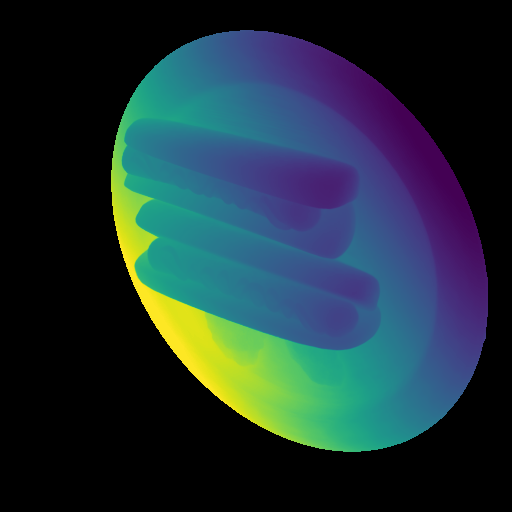
\includegraphics[width=\sw]{figures/decomp_hotdog/atlas_depth.png} &
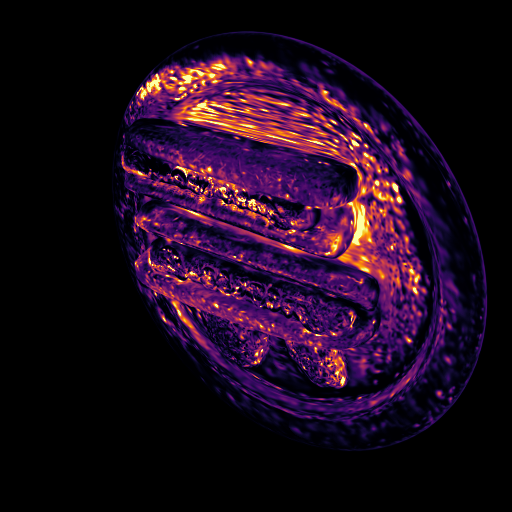
\includegraphics[width=\sw]{figures/decomp_hotdog/atlas_flux.png} &
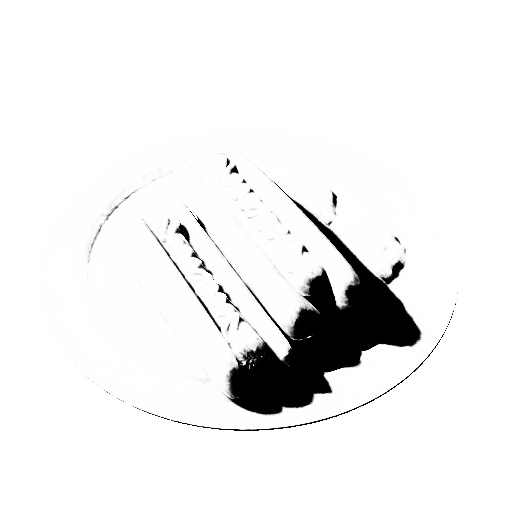
\includegraphics[width=\sw]{figures/decomp_hotdog/visibility.png} &
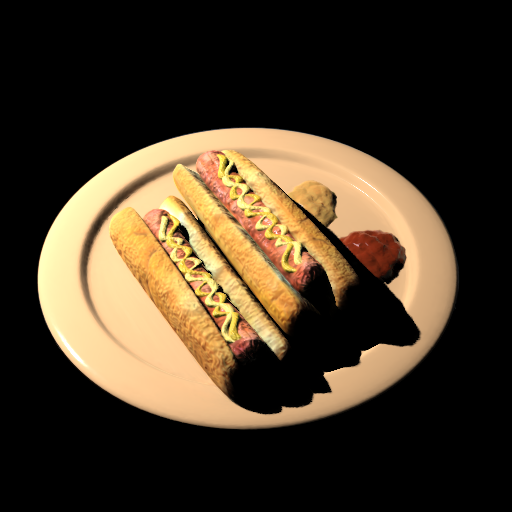
\includegraphics[width=\sw]{figures/decomp_hotdog/local.png} &
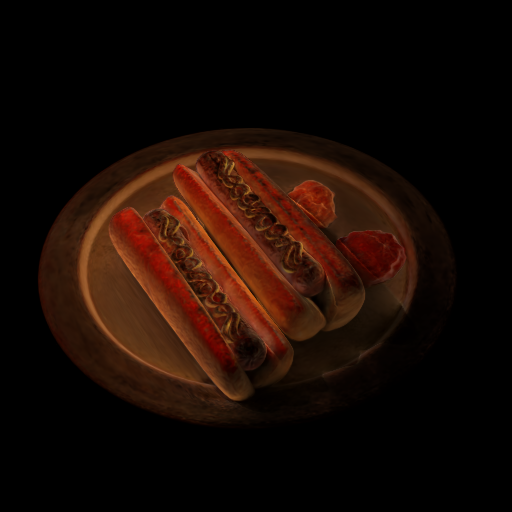
\includegraphics[width=\sw]{figures/decomp_hotdog/transfer.png} &
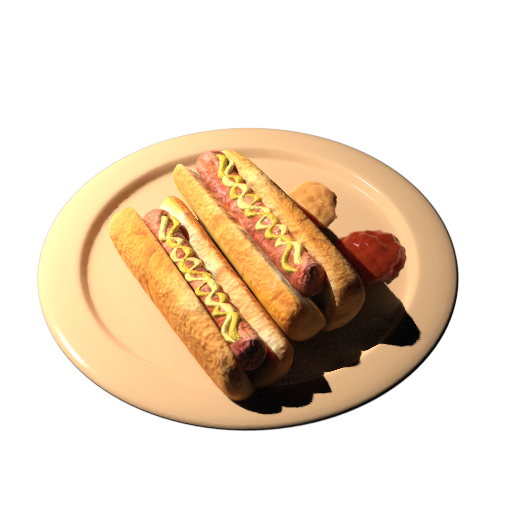
\includegraphics[width=\sw]{figures/decomp_hotdog/ours.png} &
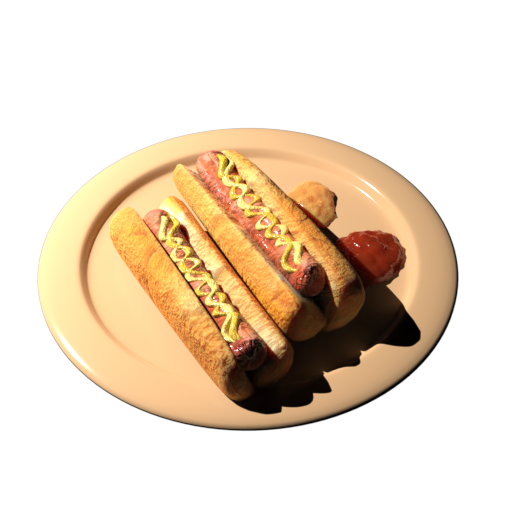
\includegraphics[width=\sw]{figures/decomp_hotdog/gt.png} \\
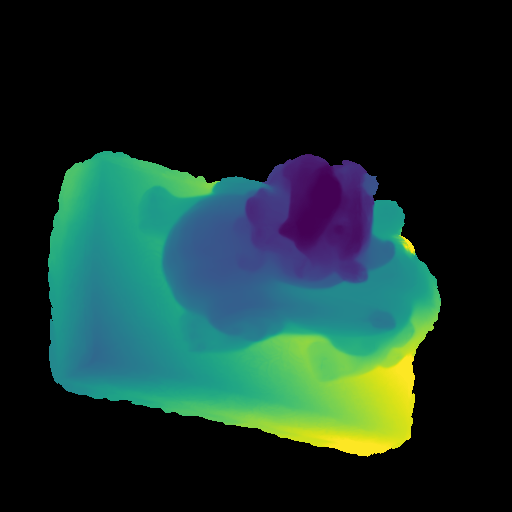
\includegraphics[width=\sw]{figures/decomp_pixiu/atlas_depth.png} &
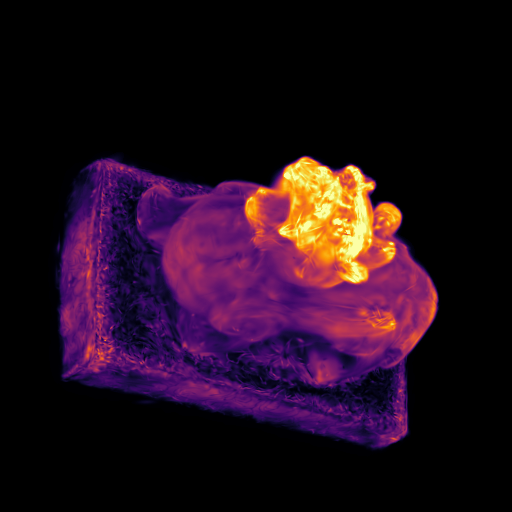
\includegraphics[width=\sw]{figures/decomp_pixiu/atlas_flux.png} &
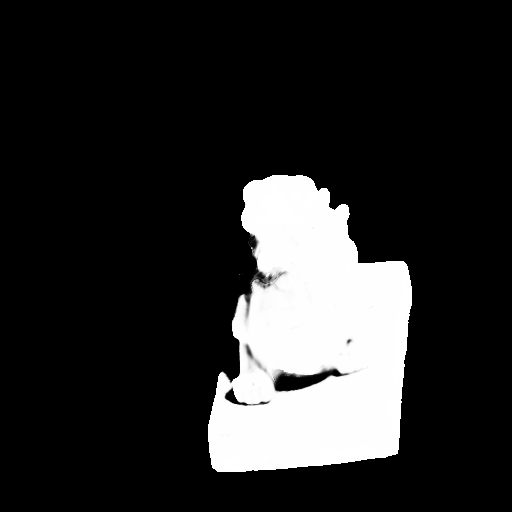
\includegraphics[width=\sw]{figures/decomp_pixiu/visibility.png} &
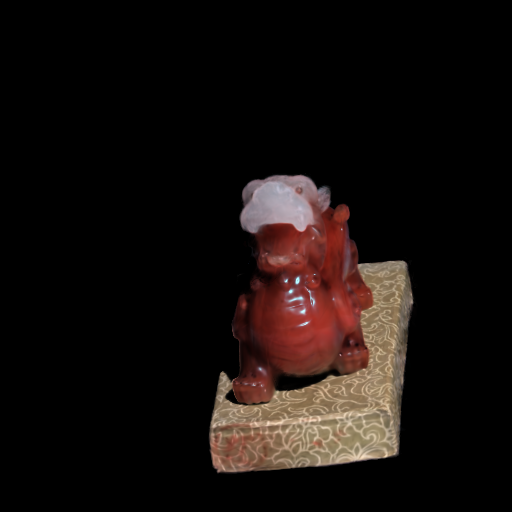
\includegraphics[width=\sw]{figures/decomp_pixiu/local.png} &
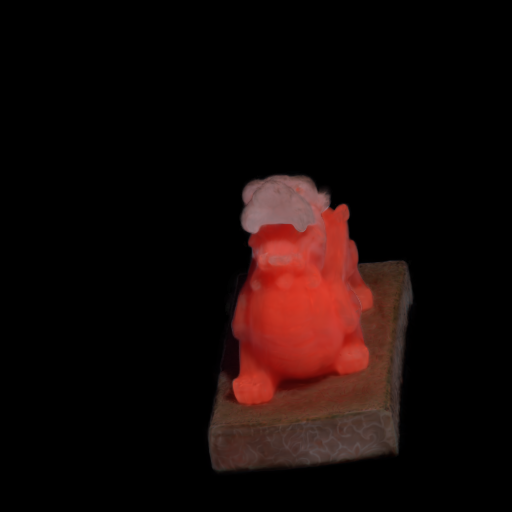
\includegraphics[width=\sw]{figures/decomp_pixiu/transfer.png} &
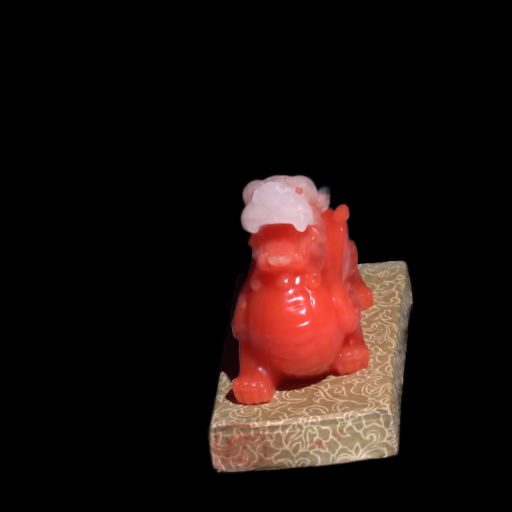
\includegraphics[width=\sw]{figures/decomp_pixiu/ours.png} &
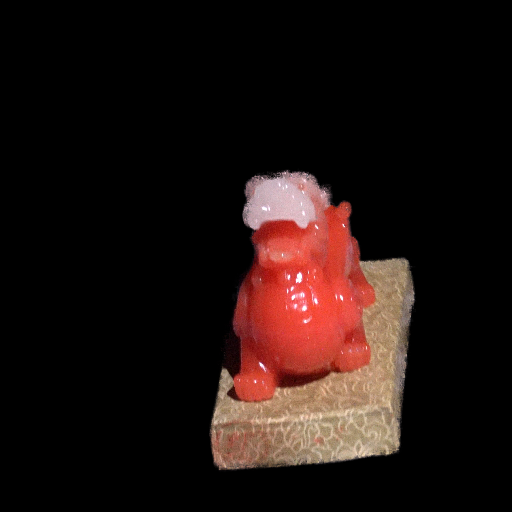
\includegraphics[width=\sw]{figures/decomp_pixiu/gt.png} \\[2pt]
\small atlas: depth & \small atlas: flux & \small visibility $V$ & \small local term & \small transfer term & \small \ours & \small ground truth
\end{tabular}
\caption{\textbf{Atlas and radiance components} of the final models on test views of Hotdog (top, 6.7\% of the radiance through the transfer term on average) and of the real Pixiu capture (bottom, a translucent resin figure, 42.1\%). On Pixiu the transfer term carries the glow of the resin, while the cast shadow on the box is explained by the visibility.}
\label{fig:s_decomp}
\end{figure*}

\begin{figure}[t]
\centering
\setlength{\tabcolsep}{0.8pt}
\renewcommand{\arraystretch}{0.5}
\newcommand{\aw}{0.242\linewidth}
\begin{tabular}{@{}cccc@{}}
\small w/o transfer & \small local residual & \small full & \small ground truth \\[2pt]
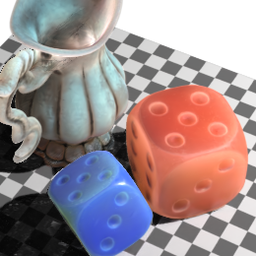
\includegraphics[width=\aw]{figures/ablation/translucent/no_transfer.png} &
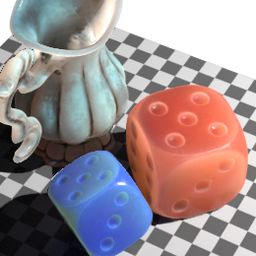
\includegraphics[width=\aw]{figures/ablation/translucent/local_residual.png} &
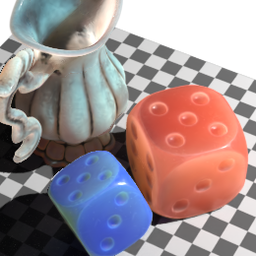
\includegraphics[width=\aw]{figures/ablation/translucent/full.png} &
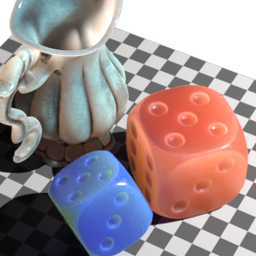
\includegraphics[width=\aw]{figures/ablation/translucent/gt.png} \\
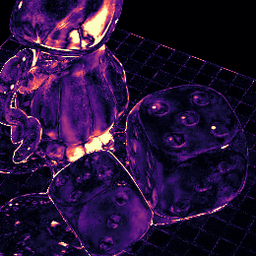
\includegraphics[width=\aw]{figures/ablation/translucent/no_transfer_error.png} &
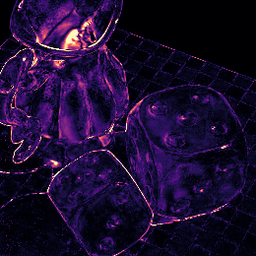
\includegraphics[width=\aw]{figures/ablation/translucent/local_residual_error.png} &
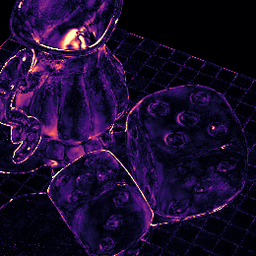
\includegraphics[width=\aw]{figures/ablation/translucent/full_error.png} & \\
\footnotesize 31.98\,dB & \footnotesize 34.55\,dB & \footnotesize 34.38\,dB & \footnotesize Translucent \\[3pt]
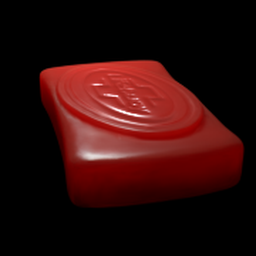
\includegraphics[width=\aw]{figures/ablation/soap/no_transfer.png} &
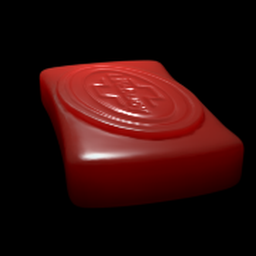
\includegraphics[width=\aw]{figures/ablation/soap/local_residual.png} &
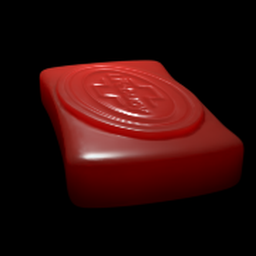
\includegraphics[width=\aw]{figures/ablation/soap/full.png} &
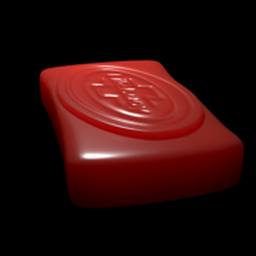
\includegraphics[width=\aw]{figures/ablation/soap/gt.png} \\
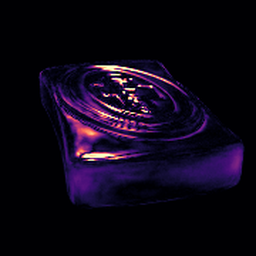
\includegraphics[width=\aw]{figures/ablation/soap/no_transfer_error.png} &
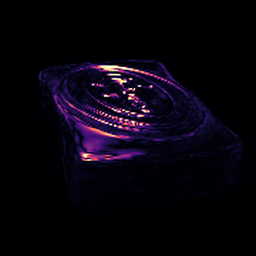
\includegraphics[width=\aw]{figures/ablation/soap/local_residual_error.png} &
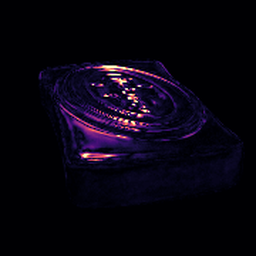
\includegraphics[width=\aw]{figures/ablation/soap/full_error.png} & \\
\footnotesize 34.66\,dB & \footnotesize 37.52\,dB & \footnotesize 37.76\,dB & \footnotesize Soap
\end{tabular}
\caption{\textbf{Transfer ablation} on the first test view of Translucent and Soap (seed 0; PSNR of the full view; error maps show the mean absolute RGB error, saturating at 0.15). Overall brightness is nearly identical across variants, but without the transfer term the errors concentrate on the translucent bodies: the blue die, the base of the vase and the sides of the soap. The local residual and the full model have similar errors, consistent with \cref{tab:paired}.}
\label{fig:s_ablation}
\end{figure}

\begin{figure}[t]
\centering
\setlength{\tabcolsep}{0.8pt}
\renewcommand{\arraystretch}{0.5}
\newcommand{\fw}{0.242\linewidth}
\begin{tabular}{@{}cccc@{}}
\small ground truth & \small \ours & \small SSD-GS & \small \gsthree \\[2pt]
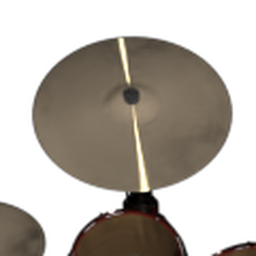
\includegraphics[width=\fw]{figures/comparison/fail_drums/GT.png} &
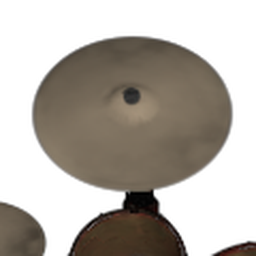
\includegraphics[width=\fw]{figures/comparison/fail_drums/LiSA-staged.png} &
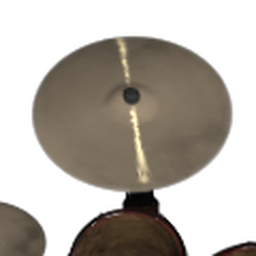
\includegraphics[width=\fw]{figures/comparison/fail_drums/SSD-GS.png} &
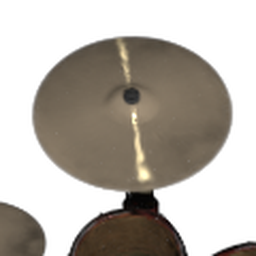
\includegraphics[width=\fw]{figures/comparison/fail_drums/GS3.png} \\
\footnotesize Drums & \footnotesize 30.90 & \footnotesize 31.32 & \footnotesize \textbf{31.93} \\[2pt]
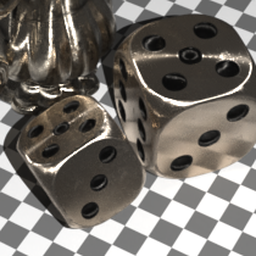
\includegraphics[width=\fw]{figures/comparison/fail_anisometal/GT.png} &
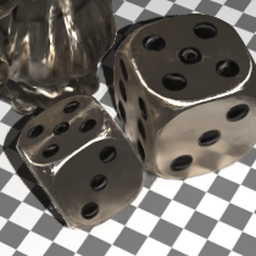
\includegraphics[width=\fw]{figures/comparison/fail_anisometal/LiSA-staged.png} &
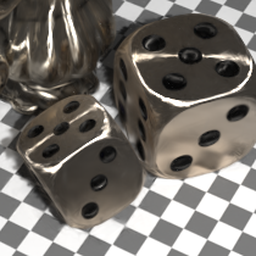
\includegraphics[width=\fw]{figures/comparison/fail_anisometal/SSD-GS.png} &
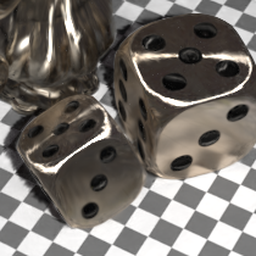
\includegraphics[width=\fw]{figures/comparison/fail_anisometal/GS3.png} \\
\footnotesize AnisoMetal & \footnotesize 27.49 & \footnotesize \textbf{28.04} & \footnotesize 27.80 \\[2pt]
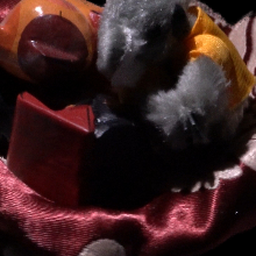
\includegraphics[width=\fw]{figures/comparison/fail_furscene/GT.png} &
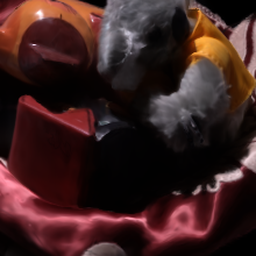
\includegraphics[width=\fw]{figures/comparison/fail_furscene/LiSA-staged.png} &
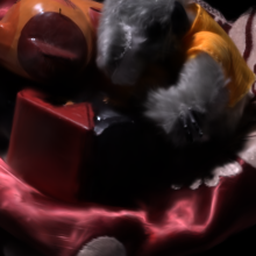
\includegraphics[width=\fw]{figures/comparison/fail_furscene/SSD-GS.png} &
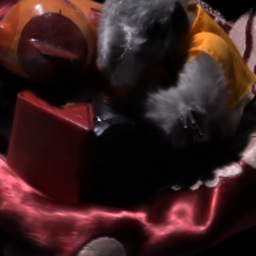
\includegraphics[width=\fw]{figures/comparison/fail_furscene/GS3.png} \\
\footnotesize FurScene & \footnotesize 24.00 & \footnotesize 24.38 & \footnotesize \textbf{25.99}
\end{tabular}
\caption{\textbf{Failure cases} at the median of the per-view margin (PSNR of the full view). \ours misses the thin anisotropic streak on the cymbal, renders the brushed-metal dice too uniformly, and loses detail in real fur.}
\label{fig:s_failures}
\end{figure}

\begin{figure}[t]
\centering
\setlength{\tabcolsep}{0.8pt}
\renewcommand{\arraystretch}{0.5}
\newcommand{\qw}{0.193\linewidth}
\begin{tabular}{@{}ccccc@{}}
\small ground truth & \small \ours & \small SSD-GS & \small \gsthree & \small OLAT-GS \\[2pt]
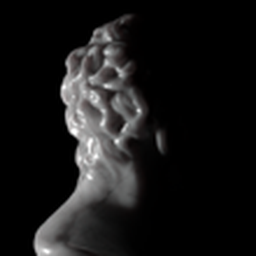
\includegraphics[width=\qw]{figures/comparison/statue/GT.png} & 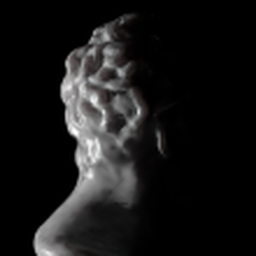
\includegraphics[width=\qw]{figures/comparison/statue/LiSA-staged.png} & 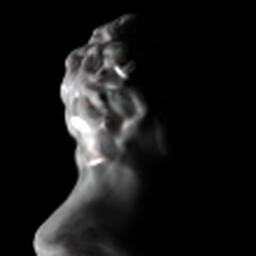
\includegraphics[width=\qw]{figures/comparison/statue/SSD-GS.png} & 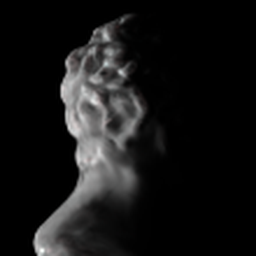
\includegraphics[width=\qw]{figures/comparison/statue/GS3.png} & 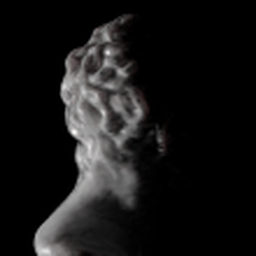
\includegraphics[width=\qw]{figures/comparison/statue/OLAT-Gaussians.png} \\
\footnotesize Statue & \footnotesize \textbf{36.23} & \footnotesize 30.90 & \footnotesize 33.51 & \footnotesize 34.16 \\[2pt]
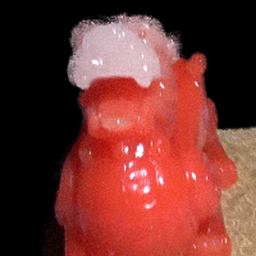
\includegraphics[width=\qw]{figures/comparison/pixiu_median/GT.png} & 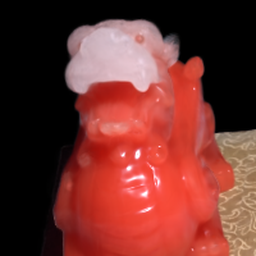
\includegraphics[width=\qw]{figures/comparison/pixiu_median/LiSA-staged.png} & 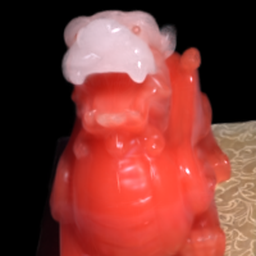
\includegraphics[width=\qw]{figures/comparison/pixiu_median/SSD-GS.png} & 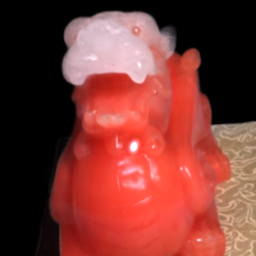
\includegraphics[width=\qw]{figures/comparison/pixiu_median/GS3.png} & 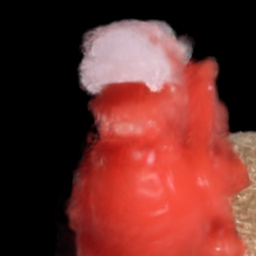
\includegraphics[width=\qw]{figures/comparison/pixiu_median/OLAT-Gaussians.png} \\
\footnotesize Pixiu & \footnotesize \textbf{26.10} & \footnotesize 23.33 & \footnotesize 23.54 & \footnotesize 21.46 \\[2pt]
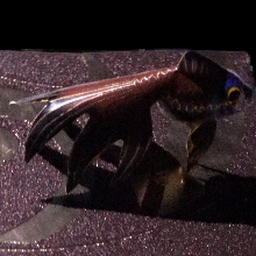
\includegraphics[width=\qw]{figures/comparison/fish/GT.png} & 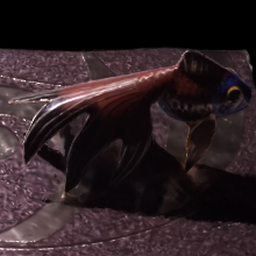
\includegraphics[width=\qw]{figures/comparison/fish/LiSA-staged.png} & 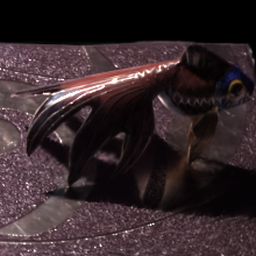
\includegraphics[width=\qw]{figures/comparison/fish/SSD-GS.png} & 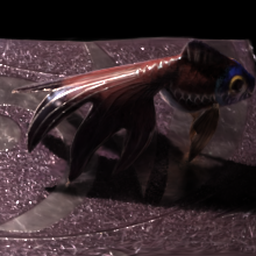
\includegraphics[width=\qw]{figures/comparison/fish/GS3.png} & 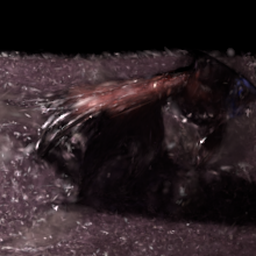
\includegraphics[width=\qw]{figures/comparison/fish/OLAT-Gaussians.png} \\
\footnotesize Fish & \footnotesize \textbf{28.18} & \footnotesize 23.38 & \footnotesize 22.26 & \footnotesize 23.40
\end{tabular}
\caption{\textbf{Further comparisons} (crops; PSNR of the full view). Statue at the 75th percentile of the per-view margin, Pixiu and Fish (real) at the median. On Pixiu and Fish the baseline crops are similarly sharp but shifted relative to the target, so much of the PSNR gap reflects registration (E2).}
\label{fig:s_more}
\end{figure}

\Cref{fig:s_decomp} shows the atlas and the radiance components for an opaque scene with strong cast shadows and for a real translucent object, and \cref{fig:s_more} further comparisons.
\Cref{fig:s_ablation} illustrates the transfer ablation of \cref{tab:ablation}, and \cref{fig:s_failures} the failure cases discussed in \cref{sec:limitations}.

\section{Experiments to be run}
\label{sec:s_torun}
The following experiments are referenced in the main paper with red placeholders.
They use the frozen final configuration; nothing is tuned on their results.

\paragraph{E1: held-out light directions.}
Partition every training set into $30^\circ$ elevation--azimuth bins of the light direction and hold out whole bins, in a fixed order, until about 10\% of the training images are held out (the deterministic split implemented in our data loader).
On the scenes we checked, this yields held-out lights $4$--$11^\circ$ (median) and up to $16^\circ$ away from the remaining training lights, compared with $0$--$2.3^\circ$ for the official test splits.
Train \ours and its local-residual variant (three seeds each) and \gsthree, SSD-GS and OLAT-GS on the remaining images of the ablation panel (Drums, AnisoMetal, Translucent, FurScene, Soap; optionally all 18 scenes), and evaluate on the held-out images with the main protocol.
Report \cref{tab:holdout}, per-scene results, paired seed differences, and per-view error against angular and camera novelty; also split by light distance, include the $\mathcal G\equiv0$ variant, and add a harder split that holds out a contiguous cap of lights at least $20^\circ$ from all training lights.

\paragraph{E2: calibration-disentangled real-scene evaluation.}
(a) Train \ours without the rotation refinement of training cameras on the seven real captures, and the baselines without pose refinement or with our gauge constraint, reporting the recovered pose offsets.
(b) For all five methods, report secondary scores after a rotation-only test-pose alignment with the scene frozen (identical for all methods) and after the best global 2D translation within 24\,px; \cref{sec:s_registration} gives the latter.
Fixed-calibration numbers remain the primary metric.

\paragraph{E3: visibility.}
Keep the receivers, schedule and atlas transfer fixed and replace the atlas shadow test by (a) per-Gaussian visibility splatted as an attribute, as in \gsthree and SSD-GS (an option of our renderer), and (b) a hard depth shadow map with percentage-closer filtering evaluated at the pixel receivers.
Also replace the Gaussian-CDF test by a Chebyshev (variance shadow map) test and sweep $\beta$, and run the single-seed rows of \cref{tab:ablation} with three seeds.
Use the ablation panel plus Hotdog, Lego and one real capture, three seeds, and report paired differences with confidence intervals; for (a), also composite per-Gaussian visibility in stage III, and for (b), use an RNG-style per-pixel depth test to separate per-pixel evaluation from moment filtering.

\paragraph{E4: optimization ablation at the full protocol.}
On the ablation panel with three seeds: (a) display-domain loss in all stages; (b) no warm-up, i.e., 30k joint iterations from the hull initialization; (c) pixel receivers in stage II; (d) no stage III, evaluating the 30k checkpoint with Gaussian receivers; (e) a display-domain loss with an offset inside $\Gamma$ or with RawNeRF-style reweighting~\cite{mildenhall2022nerf}; (f) the staged schedule applied to \gsthree or SSD-GS on LDR data.

\paragraph{E5: additional baselines.}
SSS-GS on the SSS-GS scenes once a stable reproduction under our protocol is available (the two scenes that converged can be reported now), NRHints on its real captures, and BiGS if an all-lights-on image for its initialization can be synthesized from the training data.

\paragraph{E6: baseline reproduction check.}
For each baseline, reproduce one configuration reported in its paper with the authors' protocol (resolution, image subset, background), compare with the published numbers, and inspect the low-scoring runs of RNG and OLAT-GS.

\paragraph{E7: seed variance of the main comparison.}
Three seeds for \ours on all 18 scenes, and for the strongest baseline at least on the ablation panel, to replace the single-run entries of \cref{tab:main} by means with standard deviations.

\end{document}
